% Created 2017-12-09 Sat 16:40
\documentclass[11pt]{article}
\usepackage[utf8]{inputenc}
\usepackage[T1]{fontenc}
\usepackage{fixltx2e}
\usepackage{graphicx}
\usepackage{longtable}
\usepackage{float}
\usepackage{wrapfig}
\usepackage{rotating}
\usepackage[normalem]{ulem}
\usepackage{amsmath}
\usepackage{textcomp}
\usepackage{marvosym}
\usepackage{wasysym}
\usepackage{amssymb}
\usepackage{hyperref}
\tolerance=1000
\usepackage{xeCJK}
\setCJKmainfont{宋体}
\hypersetup{colorlinks=true,linkcolor=red}
\usepackage{minted}
\usepackage{geometry}
\geometry{left=2.0cm,right=2.0cm,top=2.5cm,bottom=2.5cm}
\setmainfont{Times New Roman}
\setsansfont{Arial}
\setmonofont{Courier New}
\usepackage{indentfirst}
\setlength{\parindent}{2em}    
\author{MiracleEEEE}
\date{\today}
\title{Advanced Mathematics}
\hypersetup{
  pdfkeywords={},
  pdfsubject={},
  pdfcreator={Emacs 25.3.1 (Org mode 8.2.10)}}
\begin{document}

\maketitle
\tableofcontents


\section{多项式}
\label{sec-1}
\subsection{多项式的定义}
\label{sec-1-1}

一个以\(x\)为变量的多项式定义在一个代数域\(F\),将函数\(A(x)\)的表示为形式和:

$$
A(x)=\sum_{i=0}^{n-1} a_jx^j
$$

我们称\(a_0,a_1,\cdots,a_{n-1}\)为如上多项式的系数,所有的系数都属于域\(F\)。如果一个多项式\(A(x)\)的最高次的非零系数是\(a_k\),那么称\(A(x)\)的次数为\(k\),记入\(degree(A)=k\)。任何一个大于一个多项式系数的次数的整数都是该多项式的次数界。

\subsection{多项式的运算}
\label{sec-1-2}
\subsubsection{多项式加法}
\label{sec-1-2-1}

\includegraphics[width=.9\linewidth]{./Source/Polynomial/1.png} 

\subsubsection{多项式乘法}
\label{sec-1-2-2}

两个次数界为\(n\)的多项式的乘积为一个次数界为\(2n-1\)的多项式。

\includegraphics[width=.9\linewidth]{./Source/Polynomial/2.png}

\includegraphics[width=.9\linewidth]{./Source/Polynomial/3.png}


对于两个\(n\)次多项式乘法,朴素的多项式乘法的时间复杂度为\(O(n^2)\)。利用快速傅里叶变换算法可将时间复杂度优化到\(n\lg n\)。

\subsection{多项式的表示}
\label{sec-1-3}
\subsubsection{系数表达}
\label{sec-1-3-1}

\includegraphics[width=.9\linewidth]{./Source/Polynomial/4.png}

一般将向量作为列向量看待。

对于多项式在定点\(x_0\)的求值运算就是计算\(A(x_0)\)的值。使用霍纳法则,可以在\(O(n)\)的时间复杂度内完成求值运算。

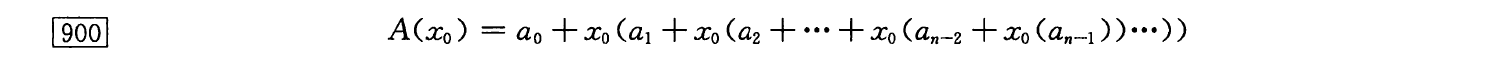
\includegraphics[width=.9\linewidth]{./Source/Polynomial/5.png}

由式子(30.2)推导出的系数向量\(c\)也称为输入向量\(a\)和\(b\)的卷积。表示成\(c=a \bigotimes b\)。

\subsubsection{点值表达}
\label{sec-1-3-2}
\begin{enumerate}
\item 点值表达的定义
\label{sec-1-3-2-1}

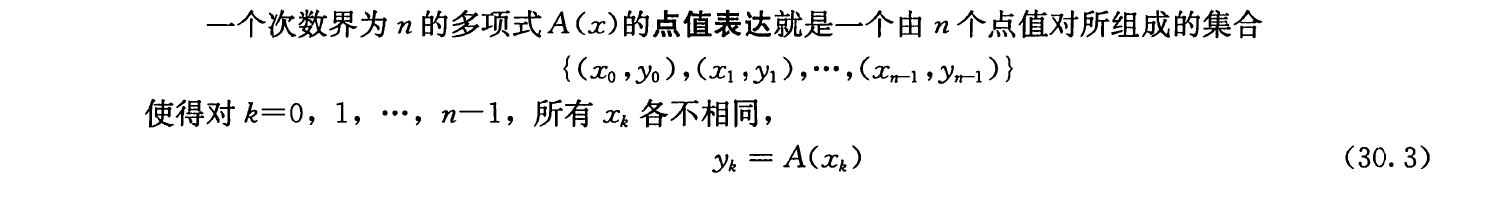
\includegraphics[width=.9\linewidth]{./Source/Polynomial/6.png}

一个多项式可以有多种点值表达。

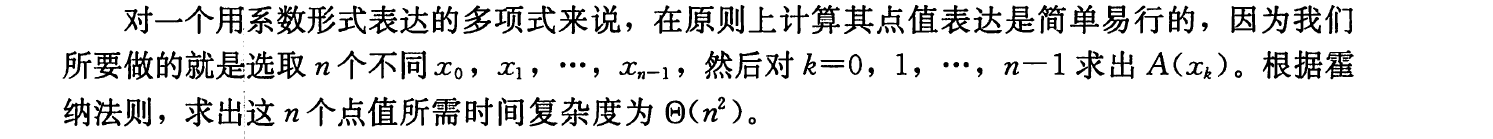
\includegraphics[width=.9\linewidth]{./Source/Polynomial/7.png}

如果选取复数单位根作为\(x_k\),就可以将其运行时间变为\(O(\lg n)\)。对于一个点值表达的多项式,求它的在某个新点上的值得最简单的办法就是先把该多项式转换成系数表达,然后在新点处求值。

\item 插值运算
\label{sec-1-3-2-2}
\begin{enumerate}
\item 高斯消元
\label{sec-1-3-2-2-1}

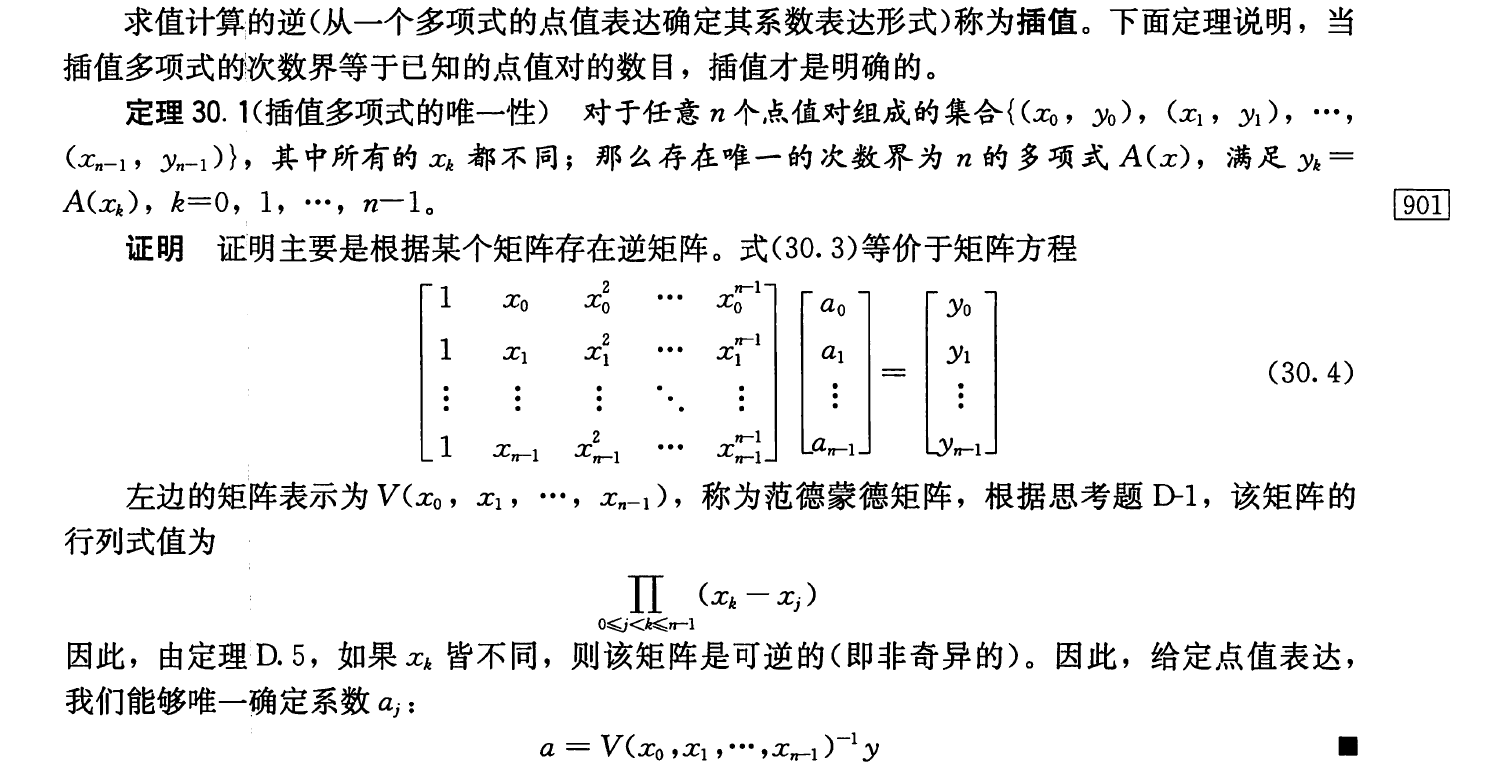
\includegraphics[width=.9\linewidth]{./Source/Polynomial/8.png}

我们可以利用高斯消元在\(O(n^3)\)的时间内求出这些方程的解。

\item 拉格朗日公式
\label{sec-1-3-2-2-2}

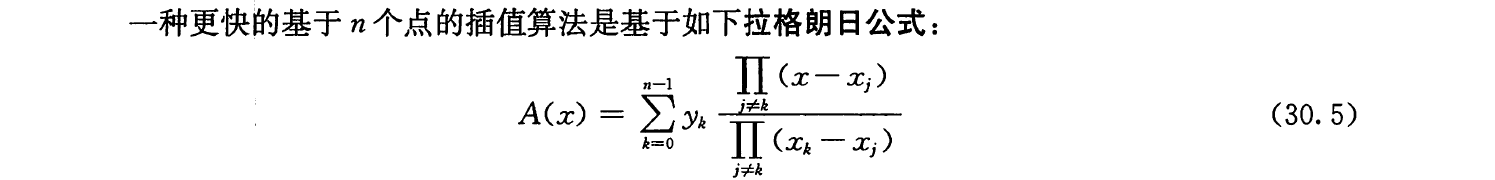
\includegraphics[width=.9\linewidth]{./Source/Polynomial/9.png}

利用拉格朗日公式可以在\(O(n^2)\)的时间复杂度内求出多项式\(A\)的所有系数。首先\(O(n^2)\)求出

$$
P(x)=\prod_j (x-x_j)
$$

然后对于每个\(k\),分子部分等于\(\frac{P(x)}{x-x_k}\),分母部分可以\(O(n)\)计算得到。

对于分子部分的计算:我们设\(A(x)=q(x)(x-x_k)+r\),\(q(x)\)为\(A(x)\)除以\((x-x_j)\)的商,为一个\(n-1\)次多项式。考虑展开:

$$
a_{n-1}x^{n-1}+a_{n-2}x^{n-2}+ \cdots +a_1x^1+a_0x^0=(x-x_k)(q_{n-2}x^{n-2}+q_{n-1}^x{n-1}+ \cdots +q_1x^1+q_0x^0)
$$

将右边乘开,整理最后得到

$$
\begin{aligned}
q_{n-2}&x^{n-1}+q_{n-3}x^{n-2}+\cdots+q_0x^1=\\
a_{n-1}&x^{n-1}+(a_{n-2}+x_kq_{n-2})x^{n-2}+\cdots+(a_1+x_kq_1)x^1+(a_0-r+x_kq_0)x^0
\end{aligned}
$$

那么:
$$
\begin{aligned}
q_{n-2}&=a_{n-1}\\
q_{n-3}&=a_{n-2}+x_kq_{n-2}\\
&\cdots\\
q_0&=a_1+x_kq_1
\end{aligned}
$$

\(q(x)\)的系数可以在\(O(n)\)的时间内求出。总的时间复杂度为\(O(n^2)\)。不过从数值稳定的角度来说,会受到较大浮点数误差的影响。
\end{enumerate}
\item 点值表达下的加法乘法
\label{sec-1-3-2-3}
\begin{enumerate}
\item 加法
\label{sec-1-3-2-3-1}

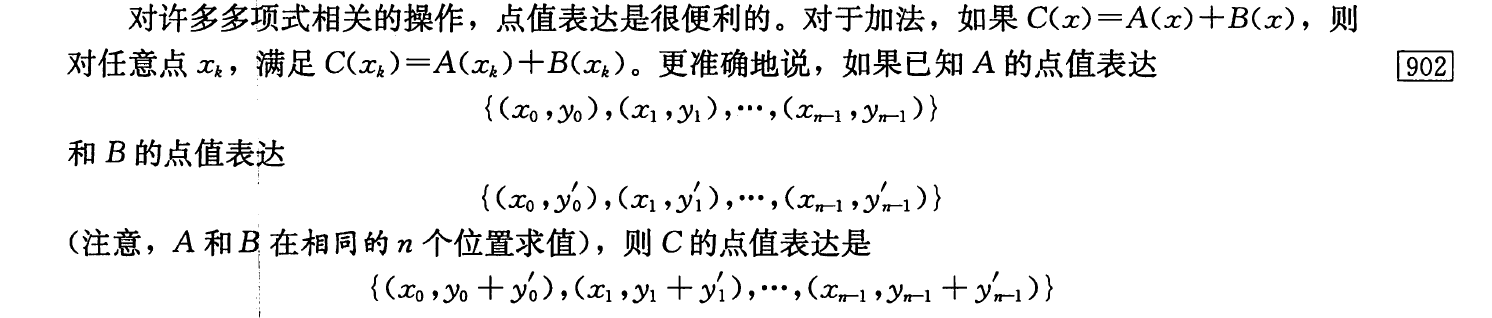
\includegraphics[width=.9\linewidth]{./Source/Polynomial/10.png}

时间复杂度为\(O(n)\)。

\item 乘法
\label{sec-1-3-2-3-2}

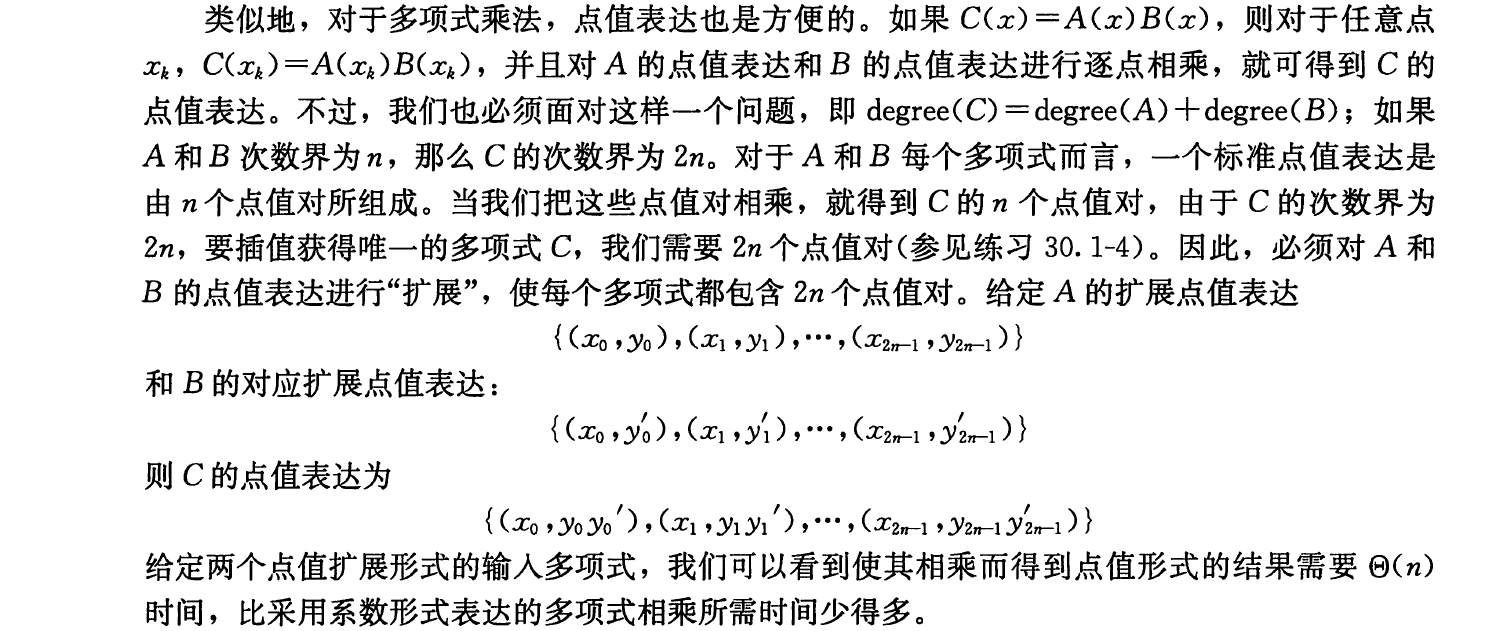
\includegraphics[width=.9\linewidth]{./Source/Polynomial/11.png}
\end{enumerate}
\end{enumerate}
\section{复数}
\label{sec-2}
\subsection{复数单位根}
\label{sec-2-1}

\includegraphics[width=.9\linewidth]{./Source/Complex/1.png}

\subsubsection{复数单位根的运算性质}
\label{sec-2-1-1}
\begin{enumerate}
\item 消去引理
\label{sec-2-1-1-1}

\includegraphics[width=.9\linewidth]{./Source/Complex/4.png}

\item 折半引理
\label{sec-2-1-1-2}

\includegraphics[width=.9\linewidth]{./Source/Complex/2.png}

这在\(FFT\)中是非常重要的。它保证了递归子问题的规模只是递归调用前的一半。
\item 求和引理
\label{sec-2-1-1-3}

\includegraphics[width=.9\linewidth]{./Source/Complex/3.png}
\end{enumerate}
% Emacs 25.3.1 (Org mode 8.2.10)
\end{document}
